\documentclass[11pt]{beamer}
\usepackage[T1]{fontenc}
\usepackage[utf8]{inputenc}
\usepackage[english]{babel}
\usepackage{mathrsfs}
\usepackage{geometry}
\usepackage{listings}
\usepackage{xcolor,graphicx}
\usepackage{xspace}
\usepackage{verbatim}
\usepackage{textcomp}
\usepackage{amsmath}
\usepackage{amsfonts}
\usepackage{syntax}
\usepackage{amssymb}
\usetheme{Boadilla}
\usecolortheme{crane}

\beamertemplatenavigationsymbolsempty

\title[Query compilation in \links]{Query compilation in\\ a functional web programming language}
\author[Gabriel Radanne]{Gabriel \textsc{Radanne}\\ {\footnotesize Under the supervision of Sam Lindley, James Cheney and Philip Wadler.}}
\institute[]{University of Edinburgh}
\date{\today}

\newcommand\mysc[1]{{\rmfamily\textsc{#1}}\xspace}
\newcommand\links{\mysc{Links}}
\newcommand\sql{\mysc{SQL}}
\newcommand\js{\mysc{Javascript}}
\newcommand\ocaml{\mysc{Ocaml}}

\newcommand\refsec[1]{\hyperref[#1]{section \ref*{#1}}}


\lstdefinelanguage{links}{
  morekeywords={var,fun,for,where},
  otherkeywords={<-,<--,=},
  morekeywords=[2]{table,database,with,from},
  classoffset=0,
  morestring=[b]",
  morecomment=[s]{/*}{*/}
}


\lstset{
  tabsize=4,
  basicstyle=\ttfamily\scriptsize,
  % upquote=true,
  aboveskip={0.5\baselineskip},
  columns=fixed,
  showstringspaces=false,
  extendedchars=true,
  breaklines=true,
  prebreak = \raisebox{0ex}[0ex][0ex]{\ensuremath{\hookleftarrow}},
  showtabs=false,
  showspaces=false,
  showstringspaces=false,
  identifierstyle=,
  keywordstyle=\color[rgb]{0.1,0.1,0.7},
  keywordstyle=[2]\color[rgb]{0.1,0.6,0.1},
  commentstyle=\color[rgb]{0.5,0.5,0.5},
  stringstyle=\color[rgb]{0.727,0.326,0.2},
}

\newcommand\sig[1]{{\tt\bf #1}}
\newcommand\code[1]{{\tt #1}}
\newcommand\linkslst[1]{\lstinputlisting[language=links]{#1}}
\newcommand\effect[1]{{\em #1}}

\newcommand\ocamlc[1]{\lstinline[language={[Objective]Caml},basicstyle=\ttfamily\normalsize]{#1}}

\newcommand\module[1]{{\bf #1}}

%comment inside bnf
\renewcommand\comment[1]{{\color{gray} $//$ #1}}


\usepackage{tikz}
\usetikzlibrary{positioning,shapes,shadows,arrows,decorations.markings,calc}
\tikzstyle{bloc}=[rectangle, draw=black, fill=yellow!20, drop shadow,scale=1.2]
\tikzstyle{etiquette}=[black!60,scale=0.8]
\tikzstyle{liaison}=[->,>=latex,very thick, rounded corners=6pt]
\tikzstyle{inter}=[<->,>=latex, double, very thick, rounded corners=6pt]

\begin{document}

\begin{frame}[plain]
\titlepage  
\end{frame}


\begin{frame}{Plan}

\tableofcontents[section]

\end{frame}


\section{What is \links ?}

\begin{frame}{What is \links}
  \links is a web functional programming language:
  \begin{itemize}
  \item Provide nice abstractions for web programming.
  \item Only one language for the client, the server and database access.
  \end{itemize}
\end{frame}


\subsection{A quick introduction to \links}

\begin{frame}[fragile]{A short example}
  A small hello example:\newline
  \begin{tikzpicture}
    
    \node (Code) at (0,0) {
      \linkslst{simplequery.links}
    } ;

    \draw<2>[thick] (-3.6,1.4) rectangle (3,0.9) ;
    \draw<3>[thick] (-3.6,0.7) rectangle (3.4,-0.1) ;
    \draw<4>[thick] (-3.6,-0.3) rectangle (3.6,-0.8) ;
    \draw<5>[thick] (-3.6,-1.0) rectangle (1.2,-1.5) ;
  \end{tikzpicture}
  
  \only<6->{And, with the right database:
  \lstinputlisting{hello-output}}
\end{frame}


\begin{frame}{\links architecture}
  \begin{figure}[htbp]
    \centering
    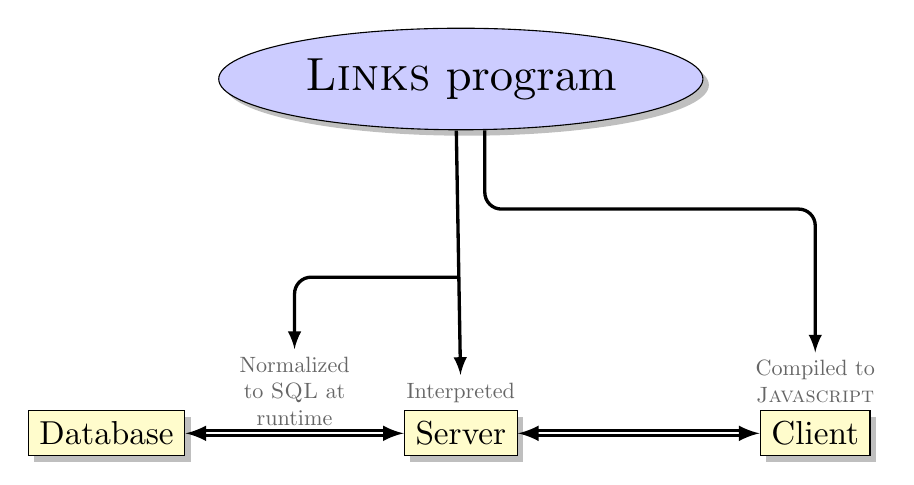
\begin{tikzpicture}[scale=1.5]
      \node[bloc,ellipse,scale=1.4,fill=blue!20] (L) at (0,3) {\links program} ;

      \node[bloc] (C) at (3,0) {Client} ;
      \node[etiquette,text centered,text width=2cm,above] (C2) at (C.north) {Compiled to \js} ;
      \node[bloc] (S) at (0,0) {Server} ;
      \node[etiquette,above] (S2) at (S.north) {Interpreted} ;
      \node[bloc] (D) at (-3,0) {Database} ;
      
      \coordinate (Lc) at (L.-65) ;
      \coordinate[yshift=-1cm] (Lci) at (Lc) ;

      \coordinate (Ls) at (L.-95) ;

      \draw[liaison] (Lc) -- (Lci) -| (C2) ;
      \draw[liaison] (Ls) -- (S2) coordinate[pos=0.6] (Ld);

      \draw[inter] (S) -- (C) ;
      \draw[inter] (D) -- (S) coordinate[pos=0.5] (DS) ;
      \node[etiquette,text centered,text width=2cm,above] (DS2) at (DS) {Normalized to \sql at runtime} ;

      \draw[liaison] (Ld) -| (DS2) ;
      
    \end{tikzpicture}
  \end{figure}

\end{frame}

\subsection{A more complex example}
\begin{frame}{A more complex example}
  \begin{tikzpicture}
    
    \node (Code) at (0,0) {
      \alt<6->{\lstset{emph={fact},emphstyle=\bf\color{red}}\linkslst{querypredicat2wrong.links}
      }{\linkslst{querypredicat2.links}}
    } ;

    \draw<2>[thick] (-4,1.8) rectangle (4,0.7) ;
    \draw<3>[thick] (-4,0.5) rectangle (3.6,-0.6) ;
    \draw<4>[thick] (-3.7,0.15) rectangle (3.6,-0.25) ;
    \draw<5>[thick] (-4,-0.8) rectangle (-0.2,-1.3) ;

    \draw<6->[thick] (-1.4,-0.85) rectangle (-0.7,-1.25) coordinate[pos=1] (F) ;

    \node<7-> (Sig) at (4,-1.05) {\color{gray}\footnotesize\sig{(Int) -\{wild\}-> Int}} ;
    \draw<7->[->,>=latex] (F.south) to[out=-30,in=-165] (Sig) ;
  \end{tikzpicture}
\end{frame}

\section{Compiling queries}

\begin{frame}{The goal}
  \begin{figure}[htbp]
    \centering
    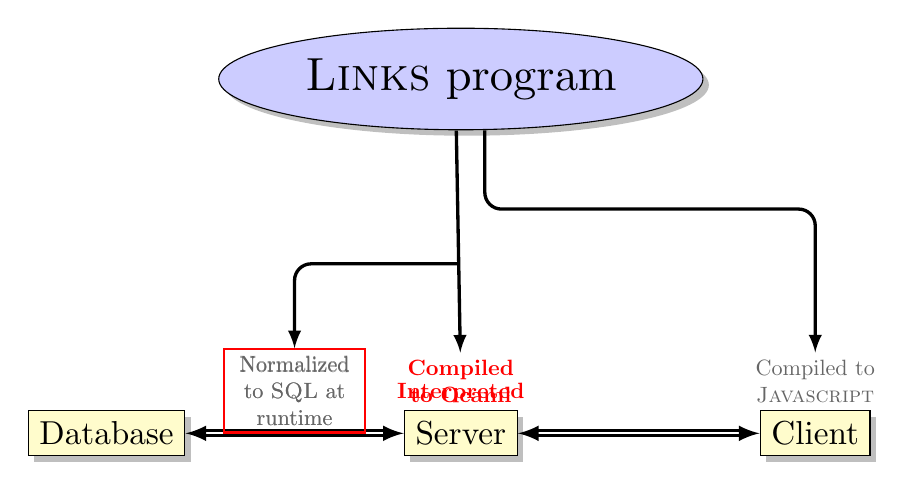
\begin{tikzpicture}[scale=1.5]
      \node[bloc,ellipse,scale=1.4,fill=blue!20] (L) at (0,3) {\links program} ;

      \node[bloc] (C) at (3,0) {Client} ;
      \node[etiquette,text centered,text width=2cm,above] (C2) at (C.north) {Compiled to \js} ;
      \node[bloc] (S) at (0,0) {Server} ;
      \node<1>[etiquette,above,red] (S2) at (S.north) {\bf Interpreted} ;
      \node<2->[etiquette,text centered,text width=2cm,above,red] (S2) at (S.north) {\bf Compiled to \ocaml} ;
      \node[bloc] (D) at (-3,0) {Database} ;
      
      \coordinate (Lc) at (L.-65) ;
      \coordinate[yshift=-1cm] (Lci) at (Lc) ;

      \coordinate (Ls) at (L.-95) ;

      \draw[liaison] (Lc) -- (Lci) -| (C2) ;
      \draw[liaison] (Ls) -- (S2) coordinate[pos=0.6] (Ld);

      \draw[inter] (S) -- (C) ;
      \draw[inter] (D) -- (S) coordinate[pos=0.5] (DS) ;
      \node<1,2>[etiquette,text centered,text width=2cm,above] (DS2) at (DS) {Normalized to \sql at runtime} ;
      \node<3>[etiquette,text centered,text width=2cm,above,draw,draw=red,thick,rectangle] (DS2) at (DS) {Normalized to \sql at runtime} ;

      \draw[liaison] (Ld) -| (DS2) ;
      
    \end{tikzpicture}
  \end{figure}

\end{frame}

\subsection{Issues}

\begin{frame}{Issues}
  Why supporting queries in the compiled file is difficult ?
  \begin{itemize}
  \item Currently, we switch interpreter at runtime and transform the AST of the code to \sql.
  \item The AST is not normally available in the compiled file.
  \end{itemize}
\end{frame}

\subsection{A solution : Doubling and Splicing}

\begin{frame}{A simple solution}
  The chosen solution is very simple :
  \begin{itemize}
  \item Double every functions : one is compiled normally and the other one contains syntactic information.
  \item Make sure value can transit from the compiled code to the syntactic one.
  \end{itemize}
\end{frame}

\begin{frame}{On the previous example}
  \begin{tikzpicture}
    
    \node (Code) at (0,0) {
      \linkslst{querypredicat2.links}
    };
    
    \draw[thick] (-4,-0.8) rectangle (-0.2,-1.3) ;
  \end{tikzpicture}
\end{frame}

\begin{frame}{On the previous example}
  \begin{tikzpicture}
    
    \node (Links) at (0,0) { \linkslst{querypredicat3.links} } ;
    \node[yshift=-2mm,etiquette, below] at (Links) {\links predicate};
    \node<2-> (PL) at (6.5,1.5) { \lstinputlisting[language={[Objective]Caml}]{predpl.ml}} ;
    \node<2->[etiquette, below] at (PL.south)  {function compiled in \ocaml};
    \draw<2->[->,>=latex] (Links) to[out=40,in=180] (PL) ; 

    \node<3-> (DB) at (6.5,0) { \lstinputlisting[language={[Objective]Caml}]{preddb.ml}} ;
    \node<3->[etiquette, below] at (DB.south)  {syntactic information};
    \draw<3->[->,>=latex] (Links) to (DB) ; 

    \node<4-> (DB) at (6.5,-1.5) { \lstinputlisting[language={[Objective]Caml}]{pred.ml}} ;

  \end{tikzpicture}
\end{frame}


\section{What about performances ?}

\begin{frame}{What about performances ?}
  Since the goal of this project was to replace an interpreter by a compiler, we need to evaluate performances.\pause
  \begin{itemize}
  \item Verify that the new support for queries do not impact performances from the original compiler.
  \item Evaluate if the compiled file with this new feature is actually faster.
  \end{itemize}
\end{frame}

\subsection{Impact on programs without queries}

\begin{frame}{Impact on programs without queries: quicksort}
  \begin{figure}[htbp]
    \centering
    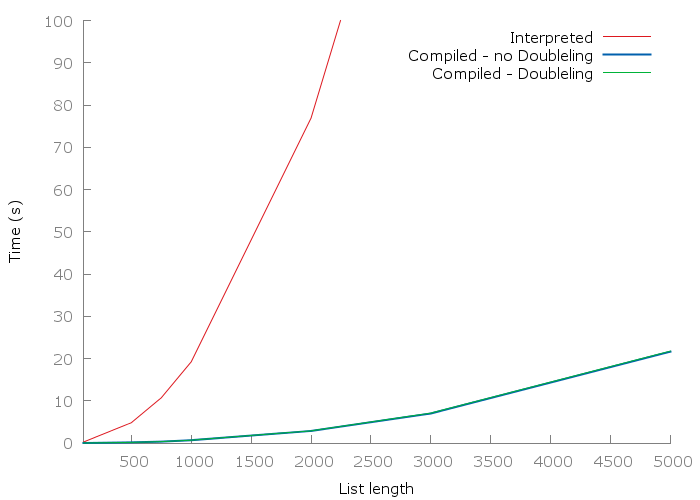
\includegraphics[width=0.7\textwidth]{quicksort.png}
  \end{figure}
\end{frame}

\begin{frame}{Impact on programs without queries: Sum on list}
  \begin{figure}[htbp]
    \centering
    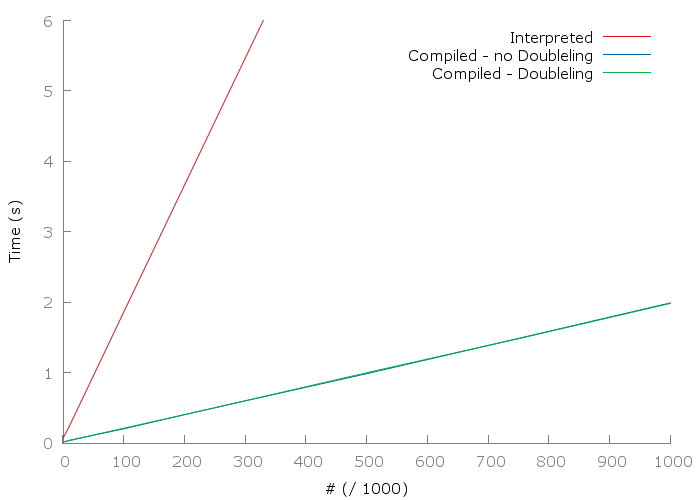
\includegraphics[width=0.7\textwidth]{sumlist.png}
  \end{figure}
\end{frame}

\begin{frame}{Impact on programs without queries: naive fibonacci}
  \begin{figure}[htbp]
    \centering
    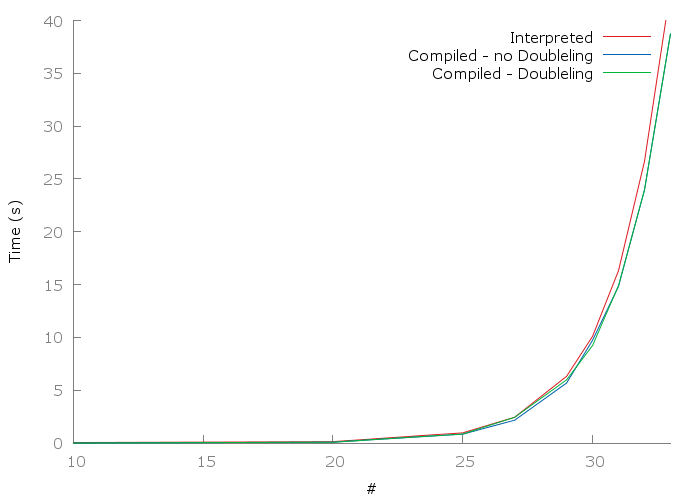
\includegraphics[width=0.7\textwidth]{fib.png}
  \end{figure}
\end{frame}

\subsection{Impact on programs with queries}

\begin{frame}{Impact on programs with queries}
Simple test protocol: repeat the hello example 10000 times.\pause
\begin{table}[htbp]
  \centering
  \begin{tabular}{|c|c|}
    \hline
    Interpreted & Compiled \\ \hline
    5.98s & 3.18s \\ \hline
  \end{tabular}
\end{table}
This is around 47\% time reduction.
\end{frame}

\begin{frame}[plain]
\begin{center}
\Huge Questions ?
\end{center}
\end{frame}

\end{document}
